

\subsection{Navier-Stokes Equation}
\label{ssec:result_nse}

\postponed{I think we should include brief results concerning \eqref{eq:nssolutionop_add} (time step to time step) as well and before the more
complicated \eqref{eq:nssolutionop2} (period to period).}

In the following section, we compare our four methods with different benchmarks on the Navier-Stokes equation introduced in subsection~\ref{ssec:nse}. The operator of interest is given by \eqref{eq:nssolutionop2}. We use the following abbreviations for the methods against which we benchmark.

\begin{itemize}
    \item {\bf ResNet:} $18$ layers of 2-d convolution with residual connections \cite{he2016deep}.
    \item {\bf U-Net:} A popular choice for image-to-image regression tasks consisting of four blocks with 2-d convolutions and deconvolutions \cite{ronneberger2015u}.
    \item {\bf TF-Net:} A network designed for learning turbulent flows based on a combination of spatial and temporal convolutions \cite{wang2020towards}.
    % The network is designed to model velocity. It may have a disadvantage on the Navier-Stokes equation formulated in vorticity form. 
    \done{I am not sure I see it this way; it is designed to approximate a solution operator and velocity versus
    vorticity is just about the space in which one studies the problem. I would move this comment somewhere else. I do understand why it is there and that it needs to be stated somewhere.}
    \item {\bf FNO-2d:} 2-d Fourier neural operator with an auto-regressive structure in time. We use the Fourier neural operator to model the local evolution from the previous $10$ time steps to the next one time step, and iteratively apply the model to get the long-term trajectory. We set and $k_{\text{max},j} = 12, d_v=32$.
    \item {\bf FNO-3d:} 3-d Fourier neural operator that directly convolves in space-time. We use the Fourier neural operator to model the global evolution from the initial $10$ time steps  directly to the long-term trajectory. We set  $k_{\text{max},j} = 12, d_v=20$.
\end{itemize}
   
\begin{figure}
    \centering
    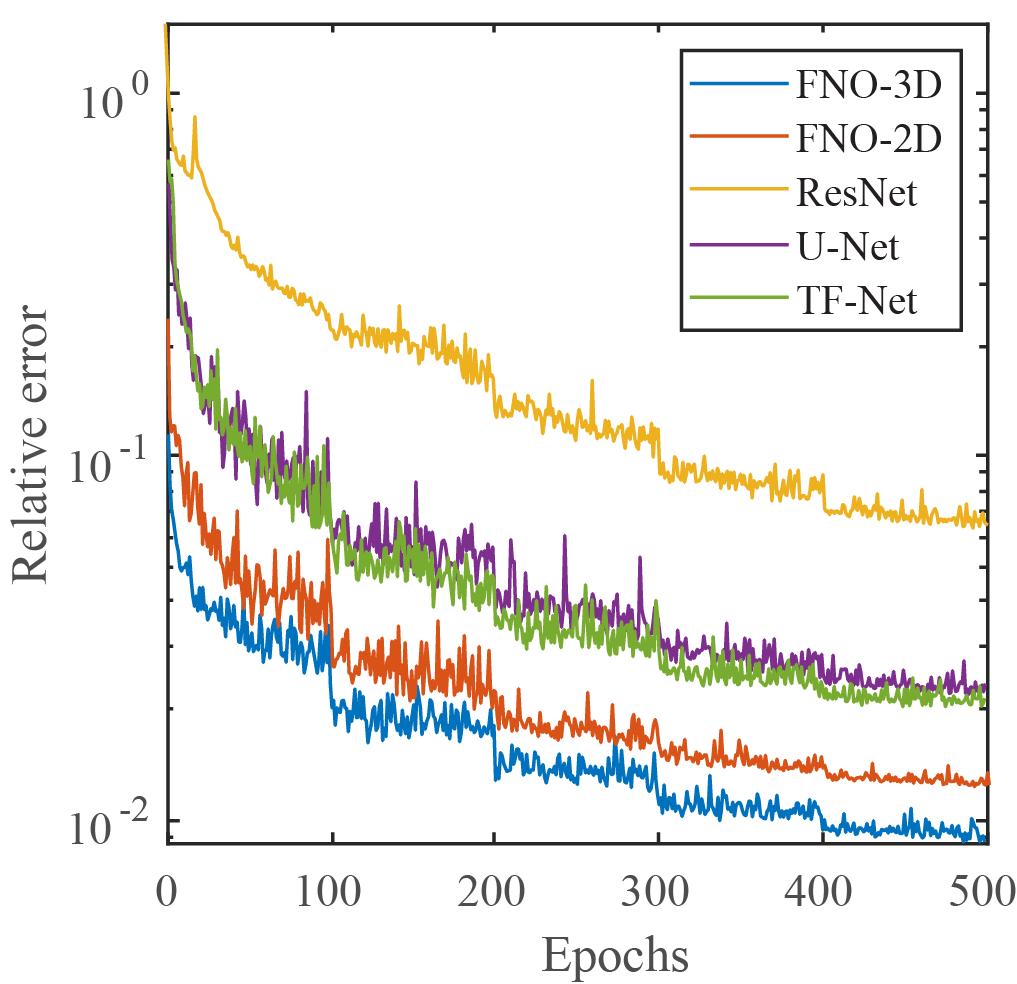
\includegraphics[width=8cm]{Figs/FourierNN_error.png}
        \caption{Benchmark on the Navier-Stokes}
    \label{fig:ns-error}
    \small{The learning curves on Navier-Stokes $\nu=1\mathrm{e}{-3}$ with different benchmarks. Train and test on the same resolution.
    For acronyms, see Section \ref{sec:numerics}; details in Tables \ref{table:ns}.} 
\end{figure}

\begin{table}[ht]
\begin{center}
\begin{tabular}{l|rc|cccc}
\multicolumn{1}{c}{} 
&\multicolumn{1}{c}{}
&\multicolumn{1}{c}{} 
&\multicolumn{1}{c}{} 
&\multicolumn{1}{c}{}\\
 & {\bf Parameters}& {\bf Time}& $\nu=10^{-3}$ &$\nu=10^{-4}$ &$\nu=10^{-4}$ & $\nu=10^{-5}$\\
 {\bf Config}&& {\bf per} &$T=50$ &$T=30$ &$T=30$ & $T=20$\\
 && {\bf epoch} &$ N=1000$ &$ N=1000$ &$N=10000$ & $ N=1000$\\
\hline 
FNO-3D    & $6,558,537$ & $38.99s$ &${\bf 0.0086}$ &$0.1918$ &${\bf 0.0820}$  &$0.1893$ \\
FNO-2D    & $414,517$ & $127.80s$ &$0.0128 $ &${\bf 0.1559}$ &$0.0834$  &${\bf 0.1556}$ \\
% \hline
U-Net       & $24,950,491$ & $48.67s$ &$0.0245 $ &$0.2051$ &$0.1190$  &$0.1982$ \\
TF-Net       & $7,451,724$ & $47.21s$ &$0.0225 $ &$0.2253$ &$0.1168$  &$0.2268$ \\
ResNet     &$266,641$ & $78.47s$ &$0.0701 $ &$0.2871$ &$0.2311$  &$0.2753$ \\
\hline 
\end{tabular}
\end{center}
\caption{Benchmarks on Navier Stokes (fixing resolution $64 \times 64$ for both training and testing).}
\label{table:ns}
% {\small The first column is the number of parameters in the network; the second column is the training time per epoch.}
\end{table}

As shown in Table \ref{table:ns}, the FNO-3D has the best performance when there is sufficient data ($\nu=10^{-3}, N=1000$ and $\nu=10^{-4}, N=10000$). For the configurations where the amount of data is insufficient ($\nu=10^{-4}, N=1000$ and $\nu=10^{-5}, N=1000$), all methods have $>15\%$ error with FNO-2D achieving the lowest among our hyperparameter search. Note that we only present results for spatial resolution $64 \times 64$ since all benchmarks we compare against are designed for this resolution. Increasing the spatial resolution degrades their performance while FNO achieves the same errors.  


\paragraph{Auto-regressive (2D) and Temporal Convolution (3D).}
We investigate two standard formulation to model the time evolution: the auto-regressive model (2D) and the temporal convolution model (3D).
\textbf{Auto-regressive models}: FNO-2D, U-Net, TF-Net, and ResNet all do 2D-convolution in the spatial domain and recurrently propagate in the time domain (2D+RNN). The operator maps the solution at previous time steps to the next time step (2D functions to 2D functions). 
\textbf{Temporal convolution models}: on the other hand, FNO-3D performs convolution in space-time -- it approximates the integral in time by a convolution. FNO-3D maps the initial time interval  directly to the full trajectory (3D functions to 3D functions). 
The 2D+RNN structure can propagate the solution to any arbitrary time $T$ in increments of a fixed interval length $\Delta t$, while the Conv3D structure is fixed to the interval $[0, T]$ but can transfer the solution to an arbitrary time-discretization. We find the 2D method work better for short time sequences while the 3D  method more expressive and easier to train on longer sequences.  

%In general the 3D method is more expressive compared to the 2D method; it is also faster and easier to train compared to the RNN structure.


\begin{table}[ht]

\begin{center}
\begin{tabular}{l|lll}
\multicolumn{1}{c}{\bf Networks}
&\multicolumn{1}{c}{\bf $s=64$}
&\multicolumn{1}{c}{\bf $s=128$}
&\multicolumn{1}{c}{\bf $s=256$}\\
\hline 
FNO-3D    & $0.0098$ & $0.0101$ &$0.0106$  \\
FNO-2D    & $0.0129$ & $0.0128$ &$0.0126$ \\
U-Net       & $0.0253$ & $0.0289$ &$0.0344$ \\
TF-Net       & $0.0277$ & $0.0278$ &$0.0301$ \\
\hline 
\end{tabular}
% \small{2D Navier-Stokes Equation with the parameter $\nu=10^{-3}$, $N=200$, $T=20$.}
\end{center}

\caption{ Resolution study on Navier-stokes equation ($\nu=10^{-3}$, $N=200$, $T=20$.)} 
\label{table:nse}
\end{table}

\subsubsection{Zero-shot super-resolution.}
\label{sec:superresolution}


The neural operator is mesh-invariant, so it can be trained on a lower resolution and evaluated at a higher resolution, without seeing any higher resolution data (zero-shot super-resolution).
Figure 
\ref{fig:super2} shows an example where we train the FNO-3D model on $64 \times 64 \times 20$ resolution data in the setting above with ($\nu=10^{-4}, N=10000$) and transfer to $256 \times 256 \times 80$ resolution, demonstrating super-resolution in space-time. The
Fourier neural operator is the only model among the benchmarks (FNO-2D, U-Net, TF-Net, and ResNet) that can do zero-shot super-resolution;
the method works well not only on the spatial but also on the temporal domain.


\begin{figure}[ht]
    \centering
    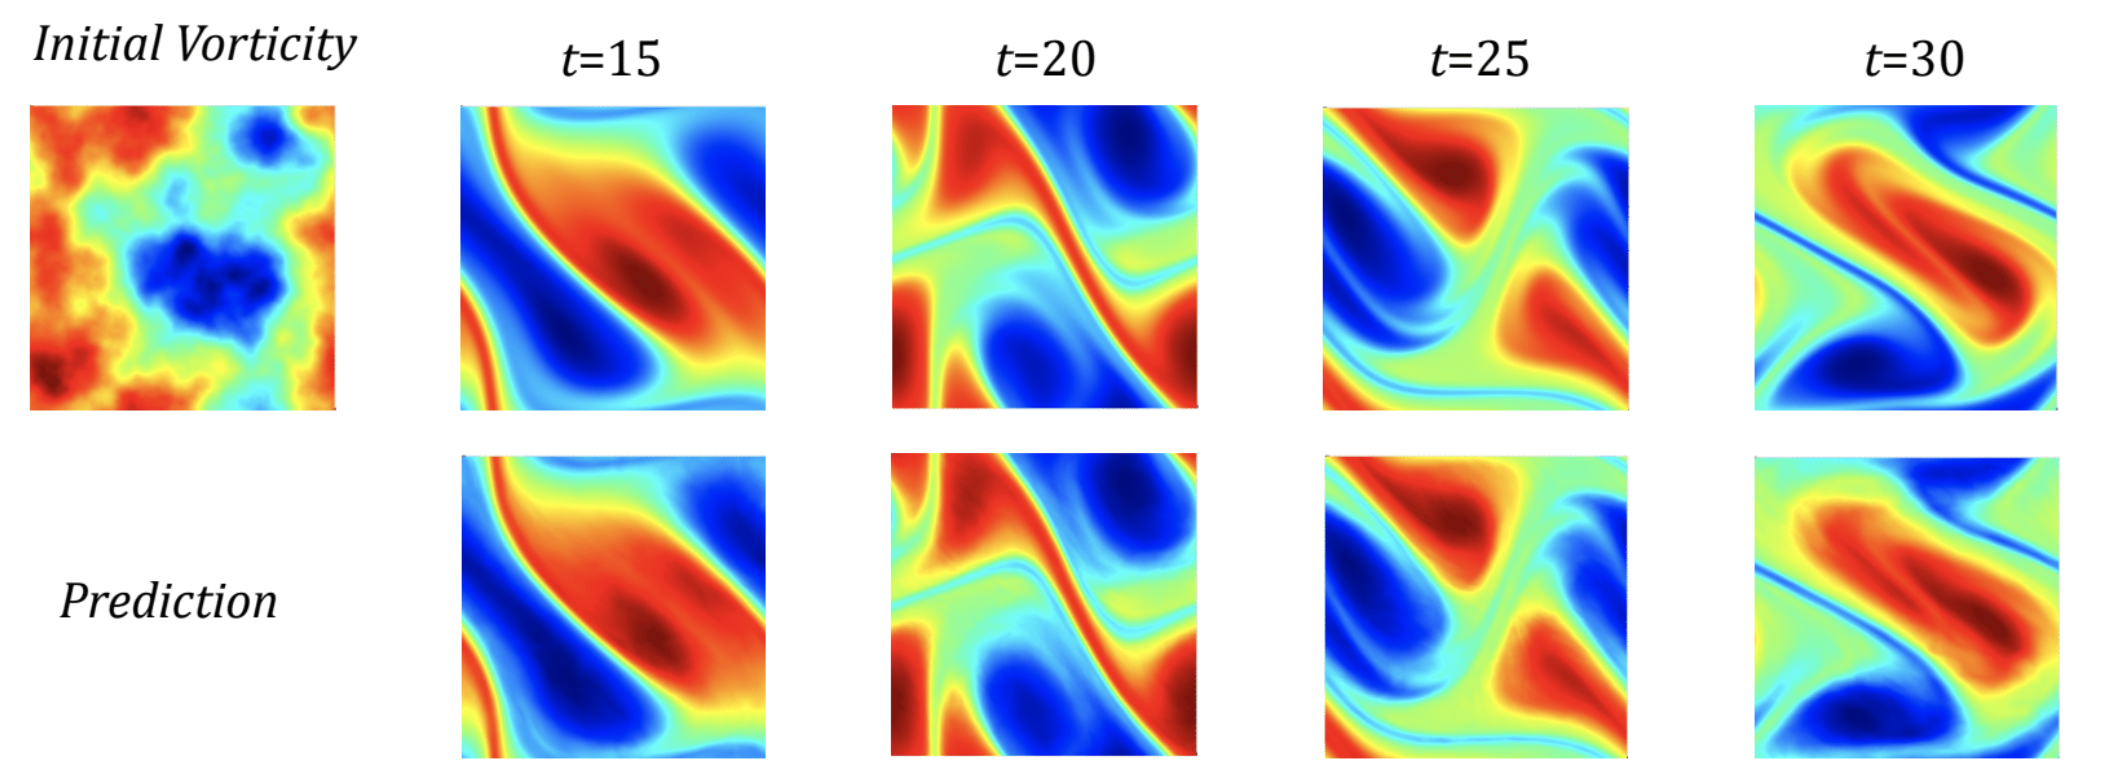
\includegraphics[width=\textwidth]{Figs/FourierNN_NV.png}
    \caption{ Zero-shot super-resolution}
    \label{fig:super2} 
    \small{ Vorticity field of the solution to the two-dimensional Navier-Stokes equation with viscosity $\nu =10^{4}$
    %\kamyar{what this means?}
    (Re$\approx200$); Ground truth on top and prediction on bottom. The model is trained on data that is discretized on a uniform $64\times64$ spatial grid and on a $20$-point uniform temporal grid. The model is evaluated with a different initial condition that is discretized on a uniform $256\times256$ spatial grid and a $80$-point uniform temporal grid. %  (see Section \ref{sec:superresolution}).
    }
\end{figure}



\subsubsection{Spectral analysis}
\begin{figure}[t]
    \centering
    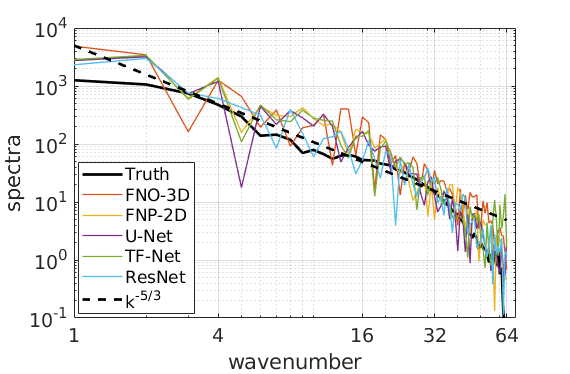
\includegraphics[width=0.48\textwidth]{Figs/spectra.png}
    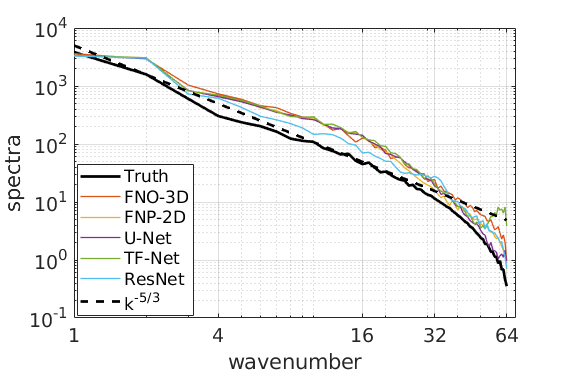
\includegraphics[width=0.48\textwidth]{Figs/spectra40.png}
        \caption{The spectral decay of the predictions of different methods}\label{fig:spectra}
    \small{
    The spectral decay of the predictions of different models on the Navier-Stokes equation. The y-axis is the spectrum; the x-axis is the wavenumber. Left is the spectrum of one trajectory; right is the average of $40$ trajectories. }
\end{figure}

\begin{figure}[t]
    \centering
    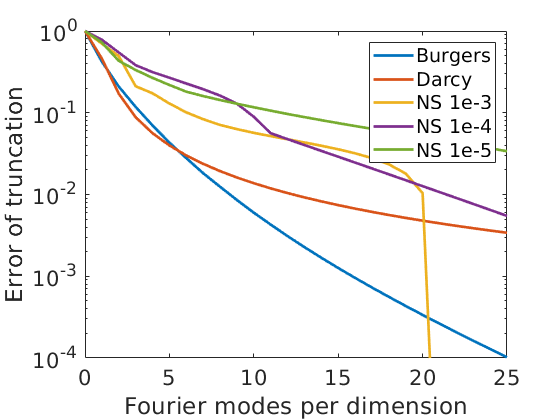
\includegraphics[width=7cm]{Figs/spectral.png}
        \caption{Spectral Decay in term of $k_{max}$ }
    \label{fig:spectral2}
    \small{ The error of truncation in one single Fourier layer without applying the linear transform $R$. The y-axis is the normalized truncation error; the x-axis is the truncation mode $k_{max}$.  }
\end{figure}

Figure \ref{fig:spectra} shows that all the methods are able to capture the spectral decay of the Navier-Stokes equation.
Notice that, while the Fourier method truncates the higher frequency modes during the convolution, FNO can still recover the higher frequency components in the final prediction. 
Due to the way we parameterize $R_\phi$, the function output by \eqref{eq:fourierlayer} has at most $k_{\text{max},j}$ Fourier modes per channel. This, however, does not mean that the Fourier neural operator can only approximate functions up to $k_{\text{max},j}$ modes. Indeed, the activation functions which occurs between integral operators and the final decoder network $Q$ recover the high frequency modes.
As an example, consider a solution to the Navier-Stokes equation with viscosity $\nu=10^{-3}$. Truncating this function at $20$ Fourier modes yields an error around $2\%$ as shown in Figure \ref{fig:spectral2}, while the Fourier neural operator learns the parametric dependence and produces approximations to an error of $\leq 1\%$ with only $k_{\text{max},j}=12$ parameterized modes.


\subsubsection{Non-periodic boundary condition.} Traditional Fourier methods work only with periodic boundary conditions. However, the Fourier neural operator does not have this limitation. This is due to the linear transform $W$ (the bias term) which keeps the track of non-periodic boundary. As an example, the Darcy Flow and the time domain of Navier-Stokes have non-periodic boundary conditions, and the Fourier neural operator still learns the solution operator with excellent accuracy.

